\documentclass[11pt]{amsart}
\usepackage[margin=1in]{geometry}
\usepackage{amsmath,amssymb,amsthm,booktabs,etoolbox,tikz}
\usepackage[T1]{fontenc}
\usepackage[utf8]{inputenc}
\usepackage{lmodern}
\usepackage[hyphens]{url}
\usepackage[colorlinks=true,linkcolor=blue,citecolor=blue,urlcolor=blue]{hyperref}
\newtheorem{theorem}{Theorem}
\newcommand{\ML}{\operatorname{ML}}
\makeatletter
\patchcmd{\@setauthors}{\MakeUppercase{\authors}}{\authors}{}{\PackageError{paper}{byline patch failed}{}}
\makeatother
\setlength{\emergencystretch}{2em}
\raggedbottom
\title{A counterexample to a lit-only sigma-game conjecture}
\author[P. Graham]{P. Graham\\ \small\url{https://orcid.org/0009-0007-8493-1505}}
\date{October 23, 2026}
\thanks{The proofs, the Lean formalization, the certificate checkers and the text were produced by AI models (from OpenAI and Anthropic), working under the author's direction.}
\hypersetup{pdfauthor={P. Graham},pdftitle={A counterexample to a lit-only sigma-game conjecture}}
\begin{document}
\begin{abstract}
A move in the sigma-game toggles the neighbors of a vertex; the lit-only
game permits such a move only at a lit vertex. The gap for a
graph is the largest difference, over starting configurations, between
the minimum numbers of lights attainable in these two games.
Goldwasser, Wang and Wu conjectured that a connected graph on $n$ vertices
with gap greater than $n/2$ must be complete $m$-partite for
$m\equiv3\pmod4$. We refute their Conjecture~5, published in 2011.
The complement of the disjoint union of a six-cycle and an isolated vertex has a starting
configuration reducible to zero lights by regular moves but to no fewer
than four by lit-only moves. A finite closed set of configurations
certifies the latter assertion. The counterexample is proved in Lean
from the definitions.
\end{abstract}
\maketitle

\section{The conjecture and the counterexample}
We define the gap between the two games, state the conjecture about large
gaps, and give a counterexample.
A configuration on a finite undirected graph $G$ assigns to each vertex
either ON (lit) or OFF (dark). Its weight is the number of lit vertices.
A regular move at a vertex toggles all its
neighbors. A lit-only move makes the same change only if the played
vertex is ON. Loops are allowed in the source convention: the played
vertex is its own neighbor exactly when it has a loop. Moves at dark
vertices do nothing in the lit-only game and may be omitted.

For a starting configuration $x$, let $\ML_G(x)$ be the least number of
lit vertices attainable by regular moves, and let $\ML_G^*(x)$ be the
corresponding lit-only minimum. These minima include the empty sequence
of moves. Following Goldwasser, Wang and Wu~\cite{GWW}, define
\[
 \mathcal D(G)=\max_x\bigl(\ML_G^*(x)-\ML_G(x)\bigr).
\]
Both minima in each difference use the same starting configuration.

\begin{theorem}\label{thm:main}
Let $G$ be the complement of the disjoint union of the six-cycle
$0,1,2,3,4,5,0$ and the isolated vertex $6$. Let $x$ have lit vertices
$\{0,1,3,4\}$. Then
\[
 \ML_G(x)=0,\qquad \ML_G^*(x)=4,\qquad
 \mathcal D(G)\geq4>\frac72.
\]
The graph $G$ is connected and is not complete multipartite.
\end{theorem}

A complete $m$-partite graph is loopless, with its vertex set partitioned
into $m$ nonempty parts, two distinct vertices being adjacent exactly when
they lie in different parts. Goldwasser, Wang and Wu's
Conjecture~5~\cite[p.~5]{GWW} starts, ``Let $G$ be a connected graph on
$n$ vertices.'' Its full implication, in mathematical form, is
\[
 \mathcal D(G)>\frac n2
 \quad\Longrightarrow\quad
 \begin{gathered}
 G\text{ is a complete }m\text{-partite graph for some positive integer }m,\\[-2pt]
 m\equiv3\pmod4.
 \end{gathered}
\]
Theorem~\ref{thm:main} contradicts that implication even for a loopless
graph. The conjecture appears in the article published
October~31, 2011~\cite{GWW}.

The contribution is the explicit graph and configuration in
Theorem~\ref{thm:main}, together with a short certificate for the
difference between their minimum light numbers. Goldwasser, Wang and Wu
studied the parameter and posed the
question, supplied the complete multipartite examples motivating it, and
reported earlier theoretical and experimental investigations
\cite[Example~4 and pp.~5--6]{GWW}. Wang and Wu's 2009
preprint~\cite{WW} studies related differences, including a difference
between two graph-wide maxima; that quantity must be distinguished from
$\mathcal D(G)$. Wu and Xiang restated the present implication in their
2019 survey and described prior experiments on lit-only reachability
\cite[Conjecture~3.3 and pp.~10--11 of the author manuscript]{WX}.
Their investigations form the background to the present question.

Nearby algebraic work includes Wu's analysis of lit-only games on line
graphs~\cite{Wu}, and Sj\"ostrand's reachability characterization,
first posted in 2023 and
published in 2025~\cite{Sjostrand}. The argument below does not require
either theory: its essential lower-bound step is to exclude every
lit-only path to a configuration of weight less than four. Exhibiting
some paths alone would not do this. A small set closed under every
allowed move supplies the exclusion.

\subsection*{Proof overview}
Section~\ref{sec:proof} specifies the adjacency lists and the starting
configuration. Two regular moves turn every light off. For the lit-only
game, a closed set contains the starting configuration and has no state
with fewer than four lights. Induction on the length of a move sequence
therefore proves the lower bound, and the starting configuration attains
it. The nonedges $01$ and $12$, together with the edge $02$, show that
nonadjacency fails transitivity and rule out every complete multipartite
graph. Section~\ref{sec:checks} describes the
Lean proof, the certificate's independent checkers, and their scope.

\section{The finite certificate}\label{sec:proof}
We give all graph and configuration data needed to prove
Theorem~\ref{thm:main}. Figure~\ref{fig:graph} shows the graph with the
starting lights. Its universal vertex~$6$ makes the graph connected.

\begin{figure}[ht]
\centering
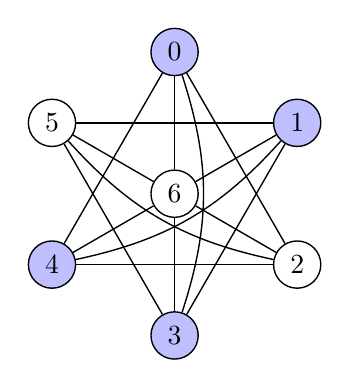
\begin{tikzpicture}[scale=0.9, every node/.style={circle,draw,
  minimum size=6mm,inner sep=0pt}, line width=0.5pt]
\node[fill=blue!25] (v0) at (0,2) {$ 0 $};
\node[fill=blue!25] (v1) at (1.73,1) {$ 1 $};
\node[fill=white] (v2) at (1.73,-1) {$ 2 $};
\node[fill=blue!25] (v3) at (0,-2) {$ 3 $};
\node[fill=blue!25] (v4) at (-1.73,-1) {$ 4 $};
\node[fill=white] (v5) at (-1.73,1) {$ 5 $};
\node[fill=white] (v6) at (0,0) {$ 6 $};
\draw (v0) -- (v2);
\draw (v0) to[bend left=18] (v3);
\draw (v0) -- (v4);
\draw (v0) -- (v6);
\draw (v1) -- (v3);
\draw (v1) to[bend left=18] (v4);
\draw (v1) -- (v5);
\draw (v1) -- (v6);
\draw (v2) -- (v4);
\draw (v2) to[bend left=18] (v5);
\draw (v2) -- (v6);
\draw (v3) -- (v5);
\draw (v3) -- (v6);
\draw (v4) -- (v6);
\draw (v5) -- (v6);
\end{tikzpicture}

\caption{The graph in Theorem~\ref{thm:main}. Filled vertices are ON in
the starting configuration $x$; open vertices are OFF.}
\label{fig:graph}
\end{figure}

For compact exact data, encode a configuration with lit set
$A\subseteq\{0,1,\ldots,6\}$ by the integer $\sum_{i\in A}2^i$.
Thus the starting configuration has code $27=1+2+8+16$.
Write $r_v$ for the code of the neighbor set of vertex $v$.
The adjacency data are
\begin{equation}\label{eq:rows}
 (r_0,r_1,r_2,r_3,r_4,r_5,r_6)
 =(92,120,113,99,71,78,63).
\end{equation}
For example, $r_0=92=4+8+16+64$ means that vertex $0$ has neighbors
$\{2,3,4,6\}$. The rows are symmetric and have no diagonal entries.
Among vertices $0,\ldots,5$, exactly the consecutive cycle pairs are
missing; vertex $6$ is universal. These are precisely the graph in
Theorem~\ref{thm:main}.

Write $a\oplus b$ for bitwise exclusive or of two nonnegative integer
codes. A regular move at $v$ sends $z$ to $z\oplus r_v$.
In particular, the regular moves $0,4$ give
\[
 27\;\xrightarrow{\;0\;}\;27\oplus92=71
 \;\xrightarrow{\;4\;}\;71\oplus71=0.
\]
No configuration has a negative number of lights, so this proves
$\ML_G(x)=0$. The second move in this sequence is unavailable in the
lit-only game, because vertex $4$ is dark in state $71$.

For the lit-only lower bound consider the set of configuration codes
\begin{equation}\label{eq:closed}
 S=\{27,45,54,63,71,78,92,99,113,120\}.
\end{equation}
The starting state belongs to $S$. Table~\ref{tab:closure} lists, for
each state, the vertices at which a lit-only move is permitted and all
their successor states. The successors in every row belong to $S$.

\begin{table}[ht]
\centering
\begin{tabular}{rll}
\hline
$z$ & Lit vertices & Successors \\
\hline
$27$ & $\{0,1,3,4\}$ & $71,99,120,92$ \\
$45$ & $\{0,2,3,5\}$ & $113,92,78,99$ \\
$54$ & $\{1,2,4,5\}$ & $78,71,113,120$ \\
$63$ & $\{0,1,2,3,4,5\}$ & $99,71,78,92,120,113$ \\
$71$ & $\{0,1,2,6\}$ & $27,63,54,120$ \\
$78$ & $\{1,2,3,6\}$ & $54,63,45,113$ \\
$92$ & $\{2,3,4,6\}$ & $45,63,27,99$ \\
$99$ & $\{0,1,5,6\}$ & $63,27,45,92$ \\
$113$ & $\{0,4,5,6\}$ & $45,54,63,78$ \\
$120$ & $\{3,4,5,6\}$ & $27,63,54,71$ \\
\hline
\end{tabular}

\caption{Closure of $S$ under lit-only moves. Successors are in the
order of the lit vertices listed in the middle column. Each is obtained
by exclusive or with the corresponding row of~\eqref{eq:rows}.}
\label{tab:closure}
\end{table}

Every lit-only state reachable from $27$ lies in $S$. Indeed, this is
true before any move; if it holds after a sequence of moves, the next
allowed move stays in $S$ by Table~\ref{tab:closure}. This proves the
claim by induction. The state $63$ has six lights and each of the other
states in $S$ has four. Consequently $\ML_G^*(x)\geq4$. The starting
state itself has four lights, so equality holds. Together with the
regular minimum this gives $\mathcal D(G)\geq4>7/2$.

Finally, $01$ and $12$ are nonedges of $G$, whereas $02$ is an edge.
In a complete multipartite graph, nonadjacent distinct vertices must lie
in the same part. The two nonedges would put $0,1,2$ in one part, in
contradiction to the edge $02$. Thus $G$ is not complete multipartite.
This completes the proof of Theorem~\ref{thm:main}.

\section{Formalization, computational checks and scope}\label{sec:checks}
The Lean project in \path{lean/} proves Theorem~\ref{thm:main} from the
game definitions, including the induction over arbitrary finite move
sequences. The theorem \texttt{LitOnlySigma.counterexample} proves the
graph's symmetry and connectivity, the two same-start minima, failure
of every complete multipartition, and the negation of Conjecture~5.
The direct refutation is also named \texttt{LitOnlySigma.not\_conjecture5}.
The definitions and their correspondence with the source are given in
\path{lean/Statement.lean} and \path{lean/FAITHFULNESS.md}.

With elan installed, the proof and its axiom guards are checked by
running the following commands from the accompanying folder:
\begin{verbatim}
cd lean
lake exe cache get
lake build
lake env lean Audit.lean
cd ..
\end{verbatim}
The toolchain and dependency manifest pin Lean and Mathlib to version
4.34.0. Finite certificate checks use kernel reduction; the proof imports
no search program or external checker. The build checks the expanded
endpoint types, the graph and starting-configuration descriptions, and
a control showing that deleting state $45$ destroys closure. Its guarded
axiom reports require exactly \texttt{propext}, \texttt{Classical.choice}
and \texttt{Quot.sound}; an additional axiom or proof hole fails the build.
The audit command replays the axiom check separately. The trusted base is
Lean's kernel and these standard logical foundations, together with the
stated identification of the definitions with the source conjecture.

The accompanying checkers verify the finite certificate used in the
proof. The file \path{data/certificate.json} contains the adjacency
rows~\eqref{eq:rows}, the starting code, the two regular moves, and the
closed set~\eqref{eq:closed}. The public check is
\begin{center}
\texttt{python3 checks/check.py}
\end{center}
It runs two independent exact checkers and corruption controls, and
confirms that the graph illustration and closure table agree with the
certificate. One checker uses integer bitmasks; the other uses explicit
sets of vertices and symmetric difference, and additionally enumerates
the configurations reachable from the starting state in each game.
Neither checker imports search code. Both reject the corrupted
certificate obtained by deleting state $45$ from~\eqref{eq:closed}.
The entry point needs Python~3.10 or later and only its standard library.
The small finite data
can also be checked directly from~\eqref{eq:rows} and
Table~\ref{tab:closure}.

The verified finite obligations are the graph's stated adjacency,
connectivity and failure to be complete multipartite; the regular path
to zero; and containment of every allowed successor of every listed
state in the listed set, with its asserted minimum number of lights.
The mathematical passage from closure to all finite lit-only move
sequences is the induction given above, also proved in Lean. The checkers
use exact integer or set operations; there is no numerical approximation.

The result concerns the exhibited starting configuration and its
consequence for the strict-threshold implication. It asserts neither
minimality of the example nor an exact graph-wide value of
$\mathcal D(G)$, and it does not settle the other light-number or
maximum-degree conjectures in the cited papers.

\begin{thebibliography}{9}

\bibitem{GWW}
J.~Goldwasser, X.~Wang and Y.~Wu,
\emph{Minimum light numbers in the $\sigma$-game and lit-only $\sigma$-game
on unicyclic and grid graphs},
Electronic Journal of Combinatorics \textbf{18}(1) (2011), P214, 27~pp.
Published October~31, 2011.
\href{https://doi.org/10.37236/701}{doi:10.37236/701}.

\bibitem{WW}
X.~Wang and Y.~Wu,
\emph{Difference between minimum light numbers of sigma-game and lit-only
sigma-game},
arXiv:0904.3050, first posted April~20, 2009.
\url{https://arxiv.org/abs/0904.3050}.

\bibitem{Wu}
Y.~Wu,
\emph{Lit-only sigma game on a line graph},
European Journal of Combinatorics \textbf{30}(1) (2009), 84--95.
\href{https://doi.org/10.1016/j.ejc.2008.02.003}{doi:10.1016/j.ejc.2008.02.003}.

\bibitem{WX}
Y.~Wu and Z.~Xiang,
\emph{The lit-only $\sigma$-game: some mathematics behind a puzzle for kids},
Mathematics Student \textbf{88} (2019), 67--98.
\href{https://ziqing.org/data/The\%20lit-only\%20sigma-game\%20-\%20Some\%20Mathematics\%20behind\%20a\%20puzzle\%20for\%20kids.pdf}{Author manuscript}.

\bibitem{Sjostrand}
J.~Sj\"ostrand,
\emph{Orbits under dual symplectic transvections},
Linear Algebra and its Applications \textbf{710} (2025), 507--530.
\href{https://doi.org/10.1016/j.laa.2025.02.010}{doi:10.1016/j.laa.2025.02.010}.
First posted December~6, 2023, as arXiv:2312.03933:
\url{https://arxiv.org/abs/2312.03933}.

\end{thebibliography}
\end{document}
